\documentclass[a4paper]{scrartcl}
% \usepackagoke{tubsdoc}
% \usepackage{float}
\usepackage[utf8]{inputenc}
\usepackage{graphicx,lipsum}
\usepackage[ngerman]{babel}

% \usepackage[format=hang]{caption}
\KOMAoption{captions}{belowfigure,nooneline}


%%%%%%%%%%%%%%%%%%%%%%%%%%%%%%%%%%%%%%%%%%%%%%%%%%%%%%%%%%%%%%%%%%%%%%%%%%%%%%%%%%%%%%%%%%%%%%%%%%%%%%%%%%%%%%%%%%%%

\author{Carsten Hoppert}
\title{Bachelorarbeit}

\begin{document}

\begin{figure}[htpb]
  \centering
  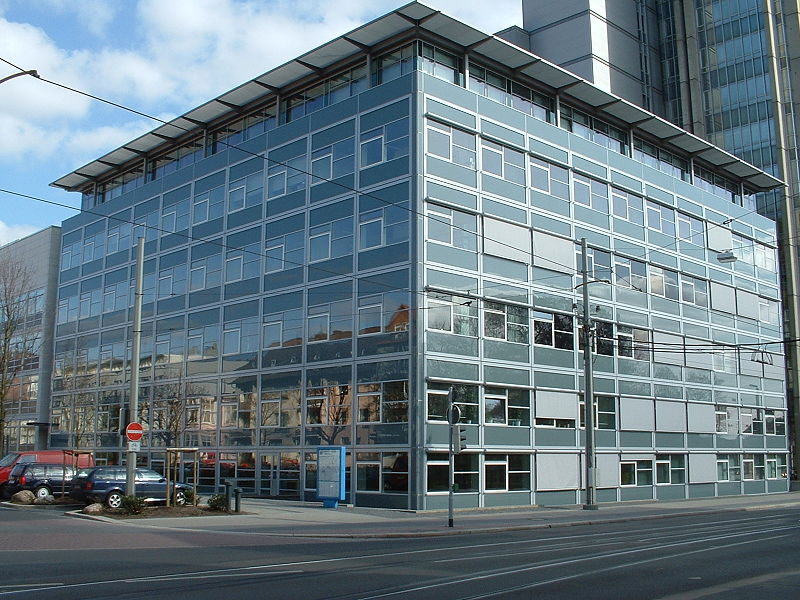
\includegraphics[width=0.5\textwidth]{infozentrum}
  \caption[Alternative]{Lorem\\ ipsum dolor sit amet amet el kun}
\end{figure}

\begin{figure}[htbp]
\centering
%1286 -> 1.286 * 1,674961119751166  ->  2,0463 => 0,8983294824399262
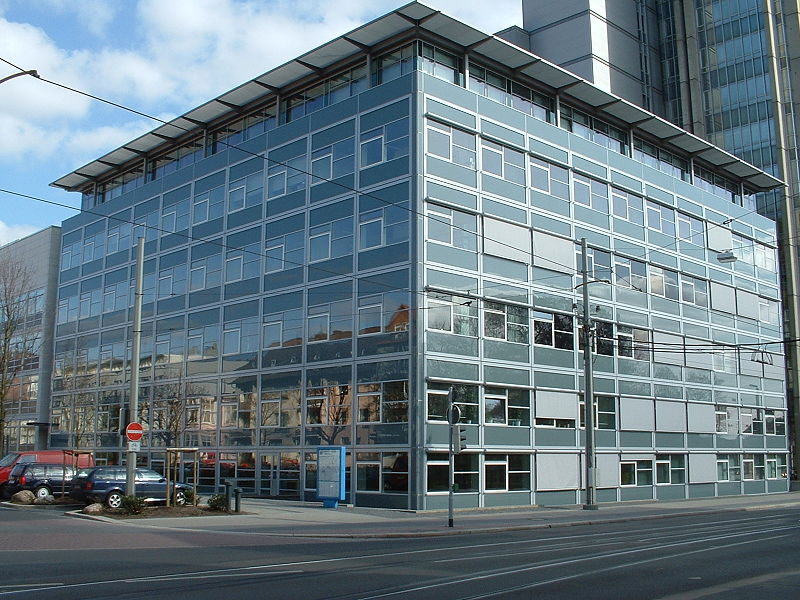
\includegraphics[width=0.8983294824399262\textwidth]{infozentrum}
\caption[Set der Feinmessplatine]{Set\\ Ausschnitt aus dem Spannungsglättung-Schaltplan (Anhang~\ref{ssec:sp_spannungsglaettung})}
\label{fig:spannungsglaettung-set}
\end{figure}% 

\end{document}
